\documentclass{standalone}
\usepackage{tikz}

\usetikzlibrary{calc,math}


\begin{document}

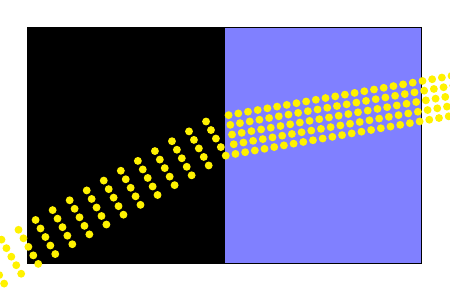
\begin{tikzpicture}
  \path[use as bounding box] (0,0) rectangle (5,3);
  \draw[fill=black] (0,0) rectangle (5,3);
  \draw[fill=blue!50] (2.5,0) rectangle (5,3);

  \foreach \i in {-10,...,7} {
    \foreach \j in {0,...,4} {
      \coordinate (P) at ($ (1,0.5) + (30:\i*0.25) + (120:\j*0.125) $);
      \path[fill=yellow] (P) circle [radius=0.05cm];
    }
  }

  \foreach \i in {1,...,30} {
    \foreach \j in {0,...,4} {
      \coordinate (P) at ($ (1,0.5) + (30:7*0.25) + (10:\i*0.125) + (100:\j*0.125) $);
      \path[fill=yellow] (P) circle [radius=0.05cm];
    }
  }

\end{tikzpicture}

\end{document}